\section{Motivating example}
%-------------------------------------------------------------------------------
The crux of the trace forensics problem is: How can we encode knowledge gained from witnessing successful executions in order to be able to to provide hints when an execution fails?

\begin{figure}[h]
\center{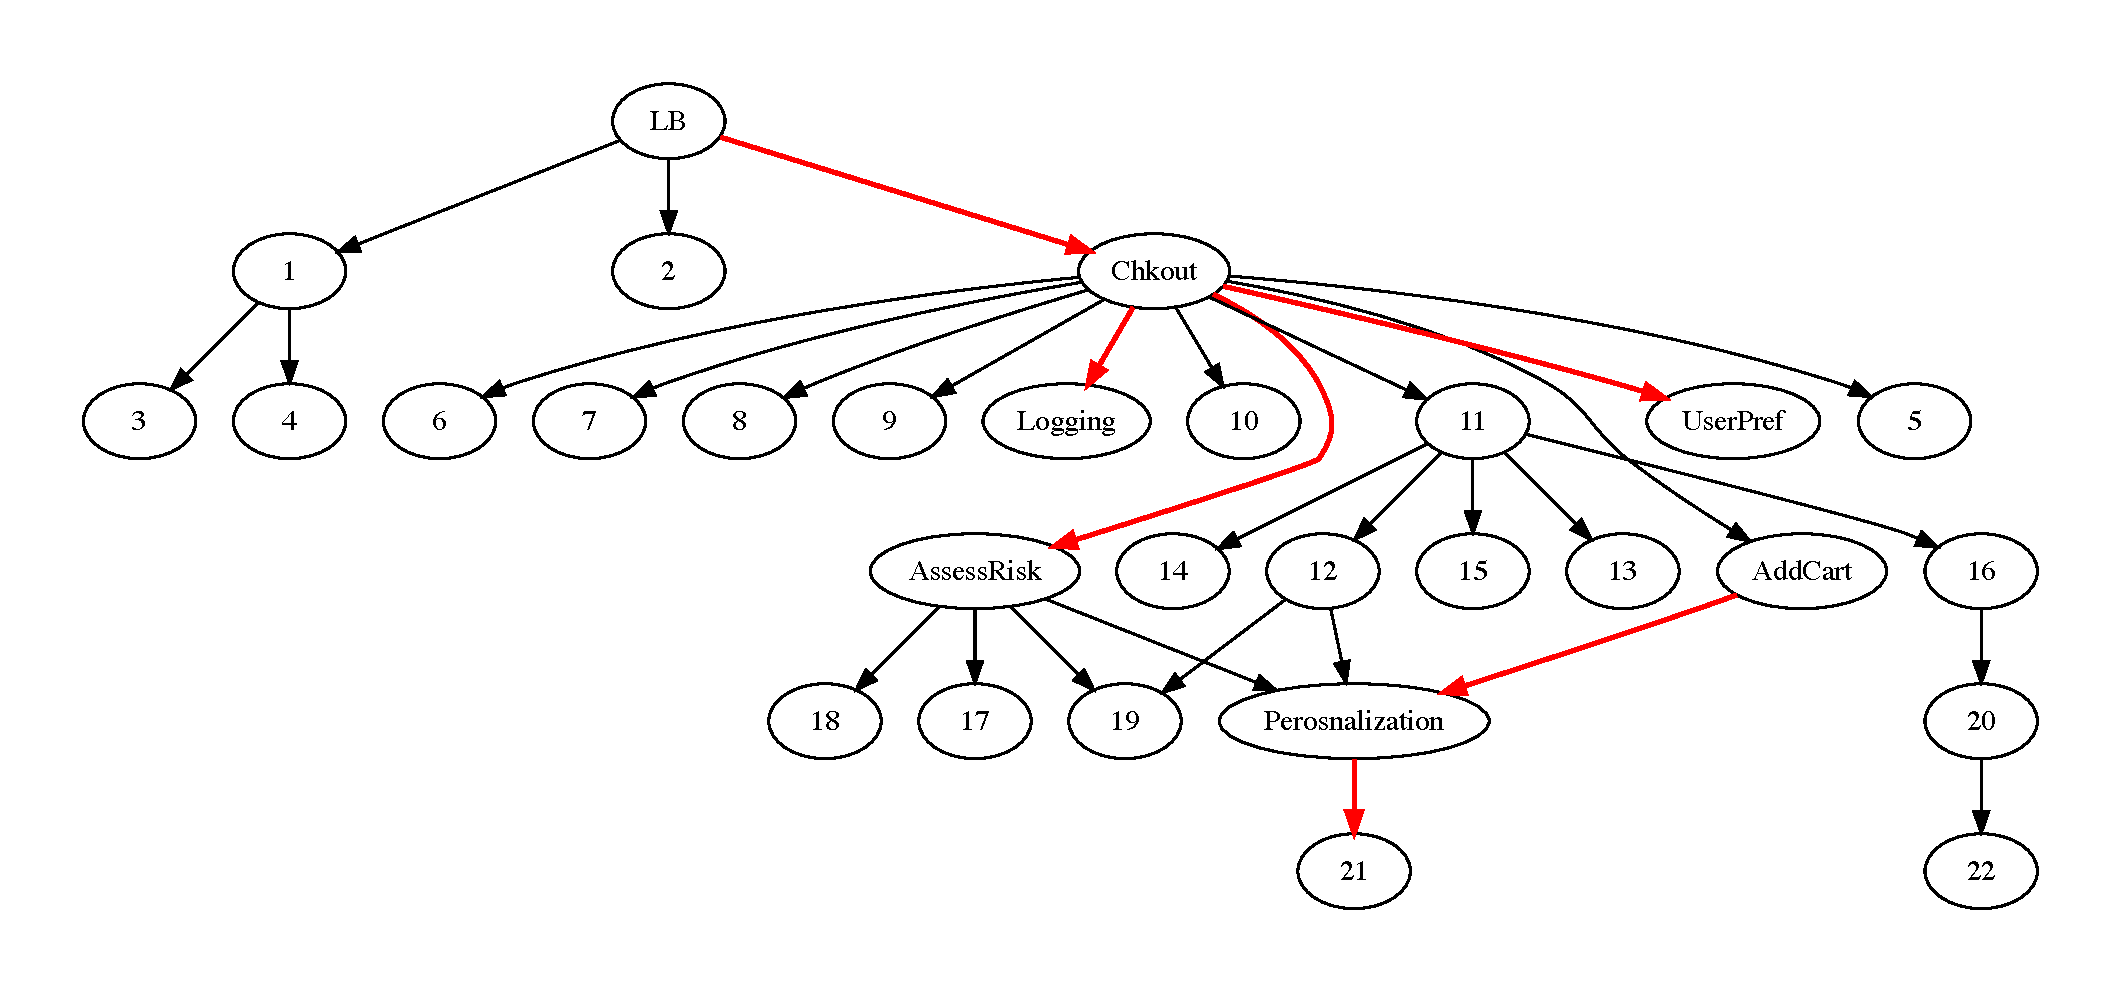
\includegraphics[scale=0.25]{anon_adrbk_fail.pdf}}
\caption{Example graph drawn from trace of a failed interaction. The red lines indicate that the callee has returned an error message to the caller}
\label{Failed_ex}
\end{figure}

Figure~\ref{Failed_ex} shows the  call-graph of a user interaction involving checkout of items for a cart for which checkout utlimately fails. The edges marked in red indicate rpc calls that were unsuccessful. The job of an SRE in this situation is to find the cause of the failure by:
\begin{itemize}
\item Figuring out which of the failures are smokescreens to be ignored. \newline
Some services that are called as part of the interaction which provide useful functionality, but the failure of which can be tolerated by the system, can be thought of as nice-to-have services. Alerts from such services may be safely ignored\ash{I think we need to say that they are not imperative for the overall successful execution and keep the ignoring or the alerts aspect out of this conversation}, the key is identifying these services and their interactions with other services. 
\item Using domain knowledge about the dependencies between services to know which alerts are the result of transitive dependencies and must be ignored. \newline
As an example, the load balancer (LB) in the figure will be alerting. An intelligent observer would conclude that since checkout (Chkout) has multiple downstream alerts, the alerts at LB are probably a result of the error being propagated up and try to dig deeper into one of the downstream alerts that look promising.
\item Determining if the absence of some services caused the failure \newline
Failures are sometimes caused by services which are required failing or a fallback path not being taken. Details of a network connection failure or time out in attempting to connect to downstream services might be buried deep in the trace. Even after we find them, figuring out the path that should have been taken but wasn't can be challenging. 
\end{itemize}
